\documentclass[12pt, letterpaper]{article}

\usepackage{graphicx}
\graphicspath{ {images/} }

\usepackage{listings}
\lstset{
	columns=fullflexible,
	breaklines=true,
	postbreak=\mbox{{$\hookrightarrow$}\space},
}

\usepackage{xcolor}

%opening
\title{Neural Network Classification of Privacy Policy Data Practices}
\author{Dr. Noriko Tomuro, August Karlstedt}

\begin{document}

\maketitle

\begin{abstract}
Privacy policies and the practices outlined in them impact every user to a given website. These policies usually include descriptions of the practices that the website operators use to collect, share, and use user data. Often unread by users because of their length and technical detail, users are unaware of how and where their data is being analyzed. We use the OPP-115 corpus of 115 privacy policies to train a neural network to classify text spans into one of ten categories in an effort to simplify these policies.
\end{abstract}

\section{Introduction}
The OPP-115 corpus is a collection of privacy policies that have been manually annotated \cite{wilson2016creation}. These annotations are a range of characters with an associated category. The possible categories include:

\begin{itemize}
\item First Party Collection/Use: how and why a service provider collects user information.
\item Third Party Sharing/Collection: how user information may be shared with or collected by third parties.
\item User Choice/Control: choices and control options available to users.
\item User Access, Edit, \& Deletion: if and how users may access, edit, or delete their information.
\item Data Retention: how long user information is stored.
\item Data Security: how user information is protected.
\item Policy Change: if and how users will be in formed about changes to the privacy policy.
\item Do Not Track: if and how Do Not Track signals 3 for online tracking and advertising are honored.
\item International \& Specific Audiences: practices that pertain only to a specific group of users (e.g., children, Europeans, or California residents).
\item Other: additional sublabels for introductory or general text, contact information, and practices not covered by the other categories.
\end{itemize}

These categories were determined by domain experts (privacy experts, public policy experts, legal scholars) \cite{wilson2016creation}. We use these categories as our target variables for our network, which we later describe in further detail. Since these categories encompass a wide range of practices, a summary of a given privacy policy could be generated with them, helping users understand its contents.

\section{Related Work}
TODO

\section{Data and Preparation Process}
The OPP-115 corpus consists 115 annotated privacy policies. For each privacy policy, users selected text spans within the document and annotated them with a single high-level category and zero or more sub-categories. An example of an annotation associated with the \textit{Third Party Sharing/Collection} category is shown in Figure 1 in JSON (JavaScript Object Notation) format.

\begin{figure}[]
\begin{lstlisting}
{
	"Third Party Entity":{
		"selectedText":"third party other than The New York Times",
		"startIndexInSegment":223,
		"endIndexInSegment":264,
		"value":"Unnamed third party"
	},
	"Choice Scope":{
		"selectedText":"null",
		"startIndexInSegment":-1,
		"endIndexInSegment":-1,
		"value":"not-selected"
	},
	"Purpose":{
		"selectedText":"participate in sweepstakes, contests or special offers.",
		"startIndexInSegment":118,
		"endIndexInSegment":173,
		"value":"Marketing"
	},
	"Choice Type":{
		"selectedText":"f you do not want any personal information shared, you should not participate in the sweepstakes, contest or special offer.",
		"startIndexInSegment":304,
		"endIndexInSegment":427,
		"value":"Dont use service/feature"
	},
	"Action Third Party":{
		"selectedText":"is also being collected by a third party other than The New York Times,",
		"startIndexInSegment":194,
		"endIndexInSegment":265,
		"value":"Collect on first party website/app"
	}
}
\end{lstlisting}
\caption{JSON annotations from the OPP-115 corpus}
\end{figure}

In this preliminary work, we generate examples of 10 higher-level categories by extracting the text spans from the sub-categories. For example, in the annotations in Figure 1, we generate multiple examples of the \textit{Third Party Sharing/Collection} category with the text spans from each sub-category, e.g.

\begin{enumerate}
	\item "third party other than The New York Times"
	\item "participate in sweepstakes, contests or special offers."
	\item "is also being collected by a third party other than The New York Times,"
\end{enumerate}

Additionally, to create a \textit{None} category that corresponds to a text span that does not deal with any data practice, we process each policy by removing all of the selected text spans as defined in the annotations. The only remaining text is then associated with the \textit{None} category and only contains text that was never selected by the user.

Figure 2 details how many examples of the 10 categories this process yields as well as how many \textit{None} examples are extracted.

\begin{figure}[h]
	\begin{tabular}{rl}
		\textbf{Count} & \textbf{Category} \\
		37299 & First Party Collection/Use \\ 
		25024 & Third Party Sharing/Collection \\
		6146 & User Choice/Control \\
		1691 & User Access, Edit and Deletion \\
		942 & Data Retention \\
		1008 & Data Security \\
		1225 & Policy Change \\
		90 & Do Not Track \\
		937 & International and Specific Audiences \\
		3544 & Other \\
		1764 & None \\
	\end{tabular}
	\caption{Number of examples of each category and the \textit{None} category}
\end{figure}

To prepare the data for the network, we encode the 10 data practice categories into one hot encoded representations.  

For the text spans, we take some normalization and preprocessing steps. First, we convert the text to lowercase. We then apply the Natural Language Toolkit (NLTK) lemmatizer. With the resulting processed text span, we build a vocabulary for a Paragraph2Vec model.

In the above proprocessing steps, we also keep track of the selected text spans in a given policy in order to generate an eleventh category for "None" -- a category where a given text span could relate to none of the possible data practices.

Finally, we train gensim's implementation of a Paragraph2Vec model on the text spans from our corpus, along with the unselected text spans that we have generated for 16 epochs.


\section{Network Setup}
The artificial neural network built here is constructed using the Keras library. Our network consists of the following layers:

\begin{itemize}
\item Fully connected layer with 256 nodes, ReLU activation
\item Dropout 25\% of the inputs
\item Fully connected layer with 256 nodes, ReLU activation
\item Dropout 25\% of the inputs
\item Fully connected layer with 11 nodes, Softmax activation
\end{itemize}

Softmax is used to produce probability distributions between the 11 possible categories and ReLU activations are Rectified Linear Units. 

Dropout is used to prevent overfitting of the training data.

We train for 128 epochs on minibatches of size 128, with a validation split of 25\%, resulting in a training set size of 59752 samples and a validation set size of 19918 samples.

\section{Results}
Results before adding the \textit{None} category were significantly better. 

\textbf{TODO: Describe them here.}

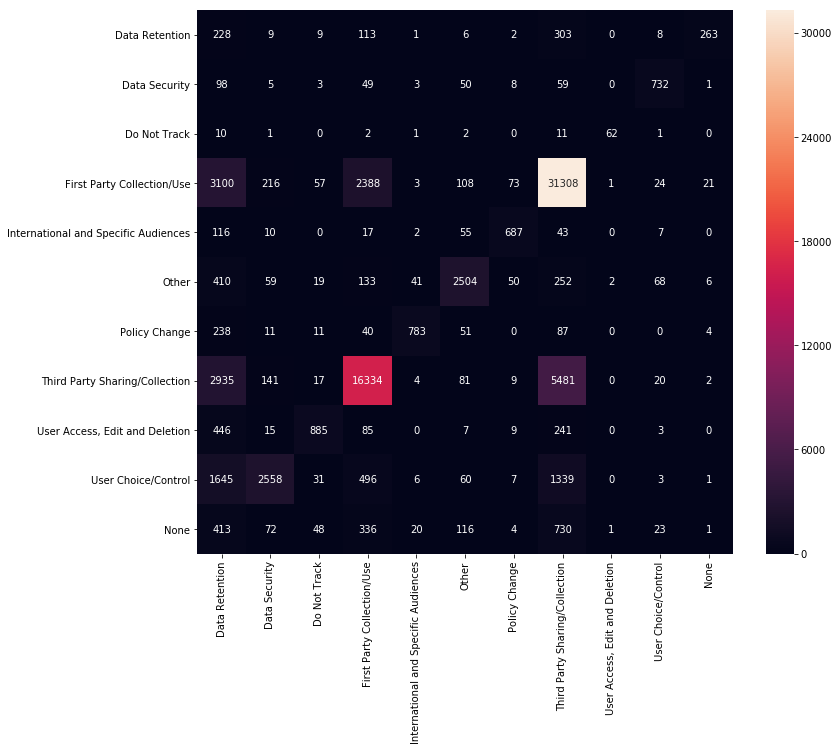
\includegraphics[width=\linewidth]{confusion-matrix}

Current results across all 11 categories results in a accuracy of 77.01\% on the training data and 51.75\% on the validation data. It is evident that the network is overfitting the training data and not learning a good representation for the mapping of training example to target. Further improvements are described in the next section.

\section{Future Work}
\begin{itemize}
\item Tweak the parameters for training the Paragraph2Vec model, e.g. number of epochs, dimensionality
\item Refine the neural network architecture
\item Perform hyperparameter tuning
\item Ensure that the text spans of the \textit{None} category do not overlap with other text spans
\item Input entire sentence or paragraph boundaries instead of just the selected text span
\item Modify the network to take advantage of recurrent neural networks since text is a sequence. It may imrpove learning of the relationships between words and categories.
\end{itemize}

\newpage
\bibliographystyle{ieeetr}
\bibliography{bibliography} 


\end{document}
